\documentclass[11pt, oneside]{article}   	% use "amsart" instead of "article" for AMSLaTeX format
\usepackage{geometry}                		% See geometry.pdf to learn the layout options. There are lots.
\geometry{letterpaper}                   		% ... or a4paper or a5paper or ... 
\usepackage{graphicx}				% Use pdf, png, jpg, or eps§ with pdflatex; use eps in DVI mode
								% TeX will automatically convert eps --> pdf in pdflatex		
\usepackage{amssymb}
\usepackage{amsmath}
\usepackage{parskip}
\usepackage{color}
\usepackage{hyperref}

\graphicspath{{/Users/telliott_admin/Tex/png/}}
% \begin{center} 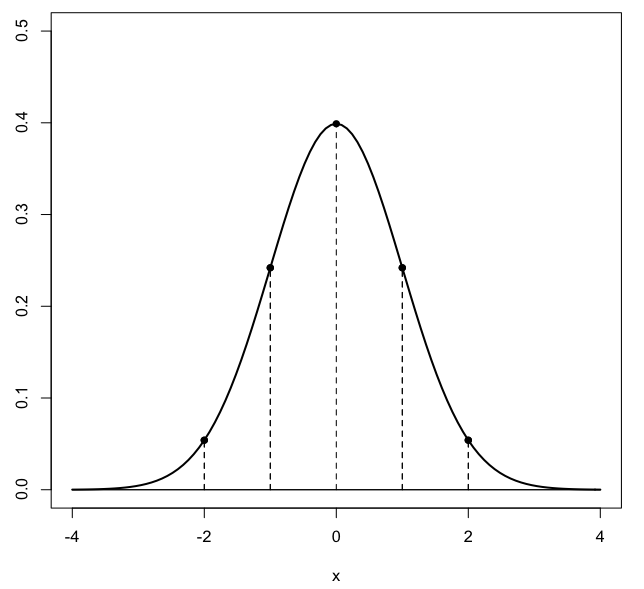
\includegraphics [scale=0.4] {gauss3.png} \end{center}

%break
\title{Paraboloid}
\date{}

\begin{document}
\maketitle
\Large


\section*{volume}

A paraboloid is a solid whose vertical cross-sections are parabolas (often oriented along the $z$-axis).

A paraboloid may open either up, or down.  
\begin{center} 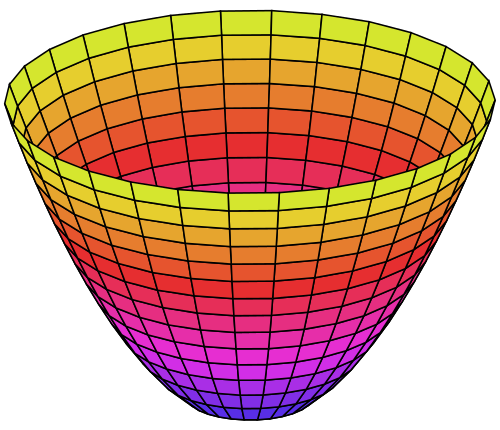
\includegraphics [scale=0.35] {paraboloid.png} \end{center}
The cross-sections parallel to the $xy$-plane are typically circles, though the shape factors for the parabolas in the $xz$- and $yz$-planes could be different, leading to an ellipse for the cross-sections.

Consider
\[ z = 2 - x^2 - y^2 \]

This is a paraboloid that opens down ($z$ gets large and negative when either $x$ or $y$ get large).  The vertex is at $z=2$.  When $z=0$, the cross-section is a circle

\[ x^2 + y^2 = 2 \]

 of radius $r=\sqrt{2}$.

Usually, cylindrical coordinates are good for dealing with this solid.  For example, in those coordinates, the surface area element is $dS = r \ dz \ d \theta$.

But let's start with a method from 1-D calculus.  Suppose we turn the paraboloid so that its symmetry axis is the $x$-axis, and its vertex is at the origin.  We can model this as being generated by revolution of the graph of $y = \sqrt{x}$ around the $x$-axis.

The general formulation is that at each point $x$, we have a circle of radius $y$ and area $\pi y^2$.  If we consider the width of each slice to be $dx$, then to get the volume just add all these up

\[ V(x) = \int A \ dx = \int \pi x \ dx \]
\[ = \pi \ \frac{x^2}{2} \ \bigg |_a^b \]

For the unit paraboloid with $a=0$ and $b=1$, we get $\pi/2$.  And our first paraboloid with $b=2$ has a volume of 

\[ V = 2 \pi \]

Now, consider the shape factor for the parabola, $a$.  In the standard equation $y=ax^2$, and the larger $a$ is, the faster the parabola grows in the $y$-direction.  But here, we have the parabola "opening" in the $+x$-direction.  That is, we have $x = a y^2$ and so $y= \sqrt{x/a}$.  Thus

\[ V(x) = \int A(x) \ dx = \pi \int \frac{x}{a} \ dx =  \frac{\pi}{a} \int x \ dx \]

and we have a factor of $1/a$ for the final volume.  

We can ask in another way if these formulas make sense.  Consider the parabola $y=x^2$ in the unit square.  The area "under" the curve is $1/3$, which is another way of saying that the area "over" the curve and inside the parabola is $2/3$.  Compare with the circle, whose area over the unit square is $\pi/4 \approx 3/4$.  The circle is a bit "fatter" than the parabola and we expect its volume, when we do the rotation, to be larger in proportion.  So this looks reasonable.

\subsection*{another method}

Let's find the volume using cylindrical coordinates.  I'd also like to generalize the problem.  In 1D we orient the vertex at the origin and integrate (usually) from $0 \rightarrow b$.  When we turn the volume so that it aligns with the $z$-axis, we usually place it with the bottom of the desired region in the $xy$-plane.  

Re-write the equation as

\[ z = f(x,y) = c - x^2 - y^2 \]

where c is the height of the parabola we are measuring.  

We are going to use $r, \theta, z$.  So we need to find the limits on $r$.  The "shadow" of the paraboloid is a circle in the $x,y$-plane 

\[ z = 0 = c - x^2 - y^2 \]
\[ x^2 + y^2 = r^2 = c \]
\[ r = \sqrt{c} \]

The volume in cylindrical coordinates is
\[ V = \iiint dV = \iiint r \ dz \ dr \ d \theta \]

What are the bounds on $z$?  Remember, if we integrate first with respect to $z$ then $r$ is \emph{fixed}.  For a given $r$

\[ z =  c - r^2  \]

So, the bounds on $z$ are $z=0 \rightarrow c - r^2$, and the inner integral is just
\[ \int_0^{c-r^2} r \ dz = r( c-r^2) \]

This gives us what we would have if we just started by thinking about the double integral of $f(x,y)$ or $f(r,\theta)$ over the region $R$ in the plane.

\[ V = \iint f(x,y) \ dx \ dy = \iint f(r,\theta) \ r \ dr \ d \theta \]

The middle integral is

\[ \int_0^{\sqrt{c}} cr - r^3 \ dr \]
\[ = \frac{1}{2}cr^2 - \frac{1}{4}r^4 \ \bigg |_0^{\sqrt{c}} \]
\[ = \frac{1}{2}c^2 - \frac{1}{4}c^2 =  \frac{1}{4}c^2 \]

times $2 \pi$ from the outer integral.  Hence $V= \pi/2 \cdot c^2$.

The way we've set up this problem, the region that we want starts at the $xy$-plane.  So there's not much point in preserving the option of starting evaluation of the middle integral at $a \ne 0$.  But if you did decide to do this you could.  Just remember to go back and fix the lower bound on $z$ in the inner integral.  That would also have to change.

Finally, we could use the method of shells.  Imagine a series of concentric cylinders with varying radius.  

Each cylinder will have height $c - r^2$ and circumference $2 \pi r$ so the lateral surface area is
\[ A = 2 \pi r (c - r^2) \]
Just integrate from 0 to well, what is the upper bound?  When $z = 0$ we have
\[ 0 = c - r^2 \]
\[ r = \sqrt{c} \]
Hence the integral is
\[ V = \int_0^{\sqrt{c}} 2 \pi r (c - r^2) \ dr \]
\[ = 2 \pi (c \frac{r^2}{2} - \frac{r^4}{4}) \ \bigg |_0^{\sqrt{c}} \]
\[ =  2 \pi(\frac{c^2}{2} - \frac{c^2}{4}) = \frac{\pi}{2} c^2 \]

The arithmetic here is exactly the same as for cylindrical coordinates, even though this is an integral of a single variable.

\subsection*{double paraboloid}

\begin{center} 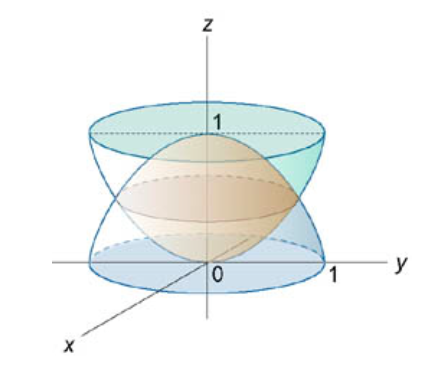
\includegraphics [scale=0.4] {doubleparab.png} \end{center}

Just for fun, let's try to do a double paraboloid.  In the figure, the paraboloid that opens up is $z= x^2 + y^2$ while the one that opens down is $z = 1-x^2 - y^2$.  To match what we had in the earlier section, I'm going to change the upper one to be $z = 2-x^2 - y^2$.

We will use cylindrical coordinates to integrate.  The key to the problem, as usual, is to find the limits for $r$ and $z$.  First, solve for the intersection of the two surfaces:

\[ z = 2-x^2 - y^2 = x^2 + y^2 \]
\[ x^2 + y^2 = 1 = r^2 \]

So $r = 0 \rightarrow 1$.  Easy enough.  And $z$ ranges from the lower surface to the upper one.  Our integral is

\[ V = \int_0^{2\pi} \int_0^1 \int_{r^2}^{2-r^2} \ dz \ r \ dr \ d \theta \]

The middle integral is

\[ \int_0^1 2 - 2r^2 \ r \ dr  \]
\[ = 2\ (\frac{r^2}{2} - \frac{r^4}{4}) \ \bigg |_0^1 \]
\[ = 2 \cdot \frac{1}{4} = \frac{1}{2} \]

Multiply by $2\pi$ from the outer integral and that gives simply, $\pi$.  Notice that we have a duplicated version of the first volume, for which we found the answer $\pi/2$.  It checks.

\subsection*{paraboloid:  surface area}

Let's do the surface area paraboloid as well.  We can write the equation as
\[ z =  c - x^2 - y^2 \]
This one opens down, and the vertex is at $z = c$.

Suppose the sign of the $c$ term is positive and we want the area above the $xy$-plane.  In the plane, $z = 0$ so
\[ x^2 + y^2 = r^2 = c \]
The radius of the circle in the plane is $\sqrt{c}$.  That will be the upper bound of the radial integral in polar coordinates.

Recall our formula
\[ dS = \ [ \ \sqrt{f_x^2 + f_y^2 + 1} \  ] \ dA \]
Here $f_x = -2x$ and $f_y = -2y$ so
\[ dS = \ [ \ \sqrt{f_x^2 + f_y^2 + 1} \  ] \ dA \]
\[ S = \int dS = \int \sqrt{1 + 4x^2 + 4y^2} \ dA \]
This is, naturally, easier in polar coordinates.  $x^2 + y^2 = r^2$ so
\[ = \int_0^{2 \pi} \int_0^{\sqrt{c}} \sqrt{1 + 4r^2} \ r \ dr \ d \theta \]

The inner integral is
\[ = \frac{1}{12} \ (1 + 4r^2)^{3/2} \ \bigg |_0^{\sqrt{c}} \]
\[ = \frac{1}{12} \ [ \ (1 + 4c)^{3/2} - 1 \ ] \ \]
Multiply by $2 \pi$ to get the whole thing.

A value for $c$ that gives a nice result is $c = 2$, then
\[ S = 2 \pi \ \frac{1}{12} \ [ \ (1 + 4c)^{3/2} - 1 \ ] \ \]
\[ = 2 \pi \ \frac{1}{12} \ (27 - 1) = \frac{26}{6} \pi \]

You can check this by computing this as a surface of revolution.  Orient the solid with its axis the same as the $x$-axis and the vertex at the origin, opening to the right.

We have
\[ y = \sqrt{x} \]
\[ y' = \frac{1}{2 \sqrt{x}} \]
The path element on the surface is 
\[ ds^2 = dx^2 + dy^2 \]
\[ ds = \sqrt{1 + y'2} \ dx \]
\[ = \sqrt{1 + \frac{1}{4x} } \ dx \]

Multiply the path element by the circumference and integrate to the same bound as we used before:
\[ A = \int 2 \pi y \ ds \]
\[ = 2 \pi \int_0^2 \sqrt{x} \ \sqrt{1 + \frac{1}{4x} } \ dx \] 
\[ = 2 \pi \int_0^2 \sqrt{x + \frac{1}{4} } \ dx \] 
\[ = \frac{4\pi}{3} (x + \frac{1}{4})^{3/2} \ \bigg |_0^2 \]
\[ = \frac{4\pi}{3} ( \frac{27}{8} - \frac{1}{8}) =  \frac{\pi}{6} \ 26 \]
which is the same as what we had before.

\end{document}